\subsection{Code}

\subsubsection{Quick start}
The code is executed by the Raspberry Pi. The python script needs to be started manually. For example, you could connect to the pi via ssh on the command line. If you know the IP address of the Raspberry Pi, you can log in via (default password is 'raspberry'): 

\begin{verbatim}
ssh pi@ipAdress
\end{verbatim}

If you don't know your Raspberry Pi's IP address, you can connect the raspberry's Ethernet cable directly to your pc. See this  \href{https://www.circuitbasics.com/how-to-connect-to-a-raspberry-pi-directly-with-an-ethernet-cable/}{Guide} or this 
\href{https://stackoverflow.com/questions/16040128/hook-up-raspberry-pi-via-ethernet-to-laptop-without-router}{Guide}. If you set up the Raspberry Pi for the first time, note the src/README.md in the \href{https://github.com/EagleEyeElite/satelliteReceiver}{git repository}. Once you are logged in, start the rotctl service:

\begin{verbatim}
source ./venv/bin/activate
cd satelliteReceiver/src/
./main.py     # start controller
\end{verbatim}

Connect to the started rotctl service from your pc:
\begin{verbatim} 
rotctl -m 2 -r 10.42.0.101:4533
\end{verbatim}


\subsubsection{Code structure}

The code implements the rotctl server. It's multithreaded to serve the clients requests and oversee the rotator simultaneously. The rotator uses two magnetic encoders, connected to the differential, to gain absolute position (even after power cut off). The motor's encoder are used to monitor the motor speed. Additionally, the rotor can observe three safety switches to cut off the motors to prevent the rotator damaging itself.
The code structure represents the structure of the rotator and the electronics. All IC's like the h-bridge, the i2c multiplexer etc. have their own driver modules. The rotator itself and the two shafts connected to the differential are also represented as objects. Note \ref{Code_structure} to see the full code structure:


\begin{figure}[H]
	\centering
	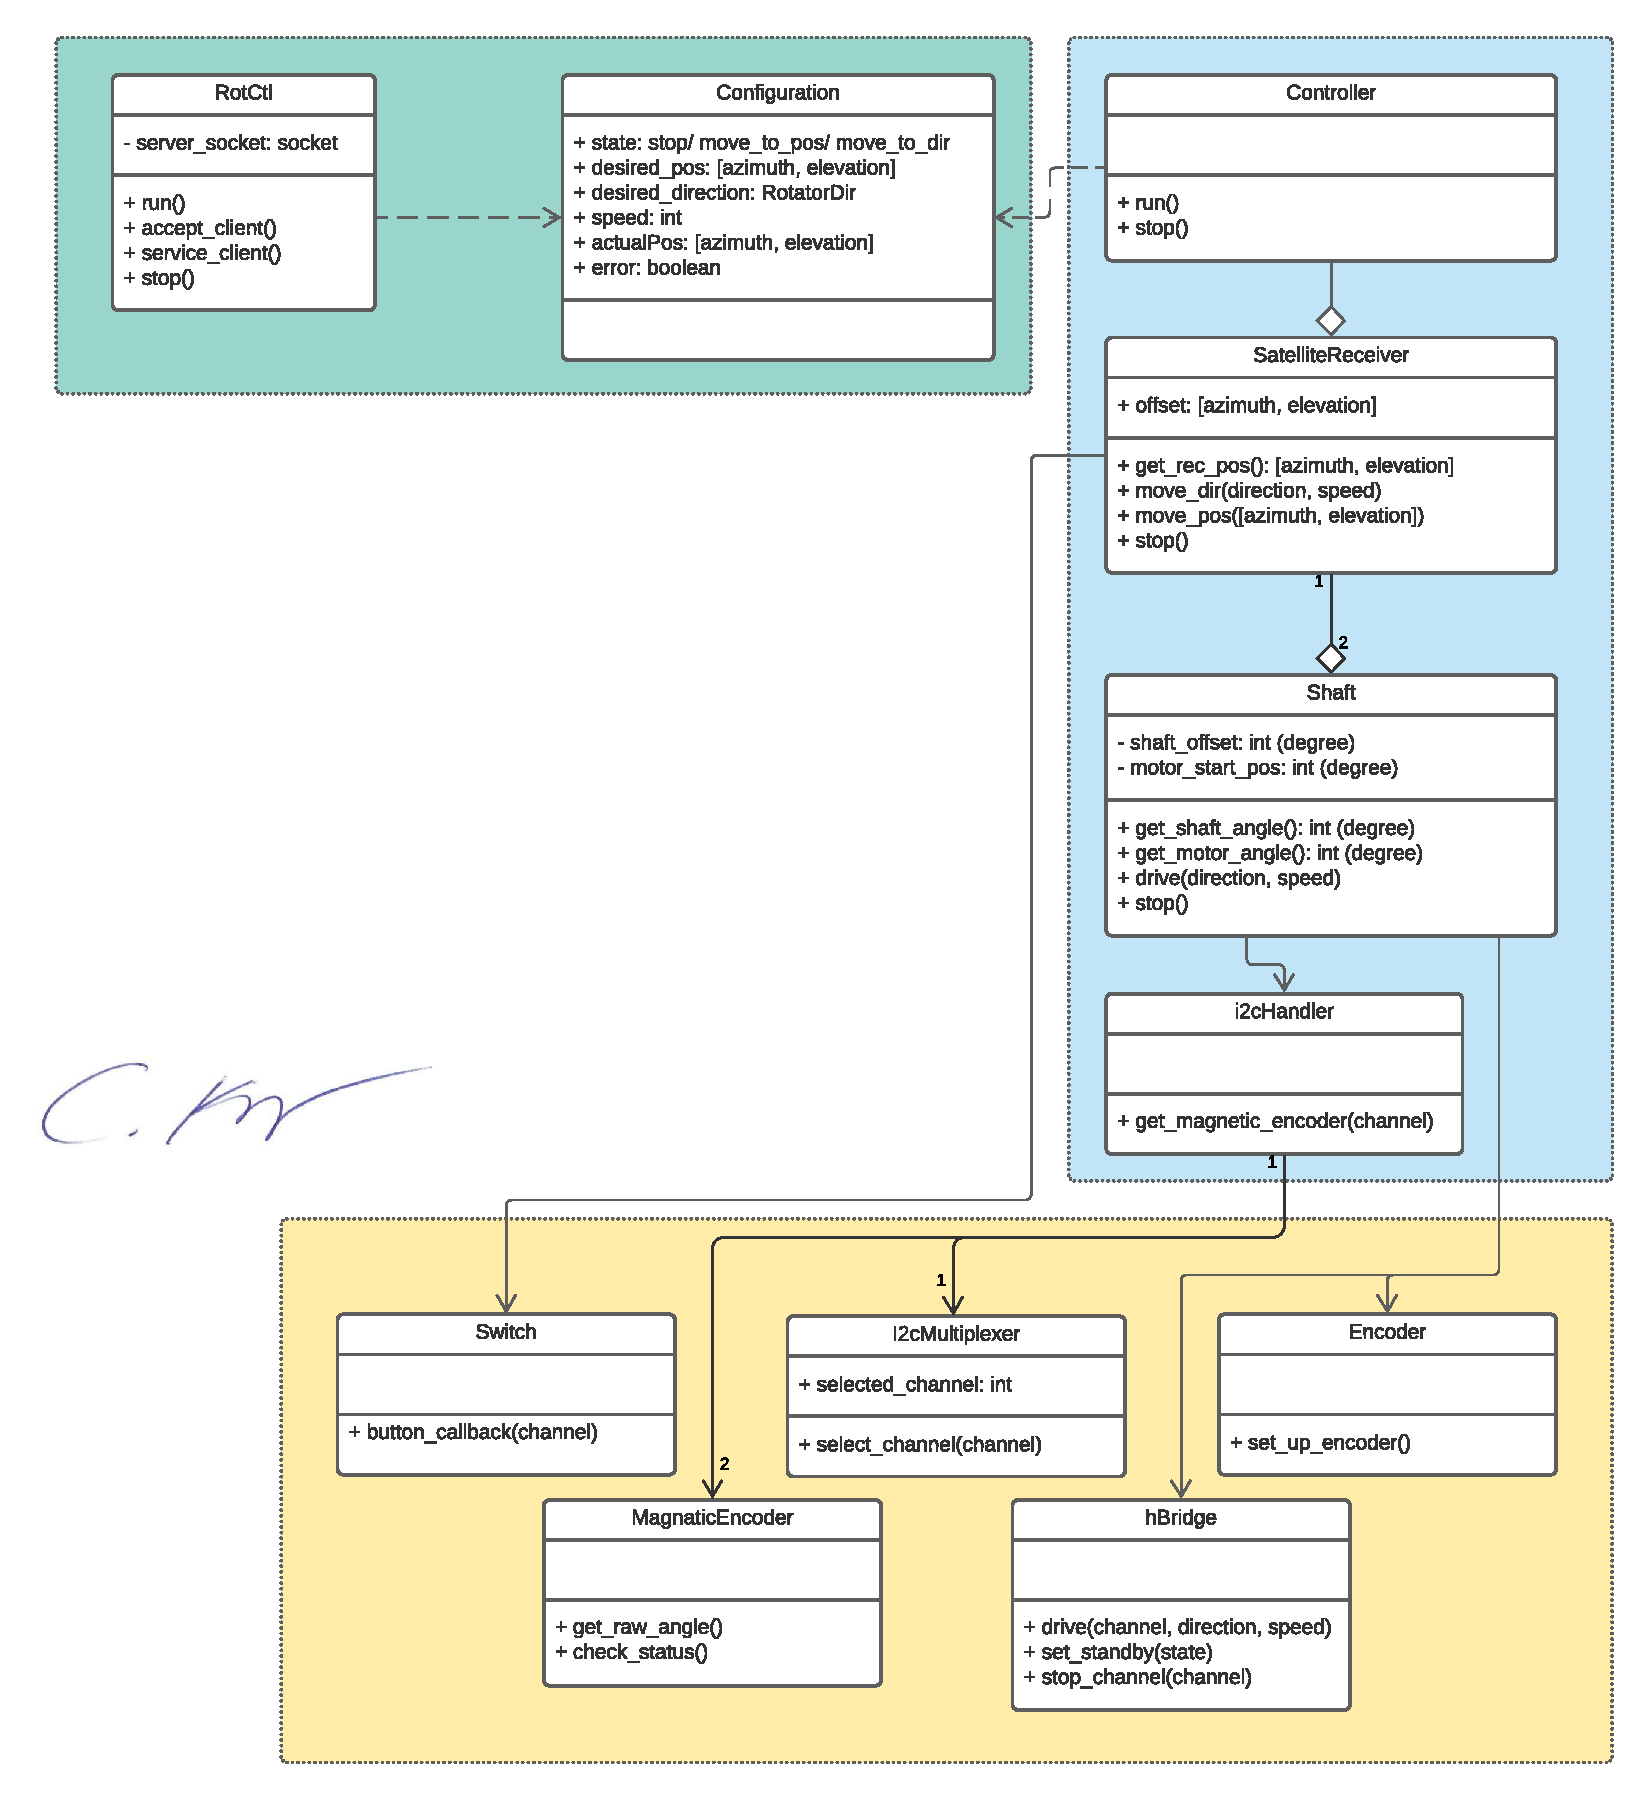
\includegraphics[scale=0.5]{../art/SatelliteReceiver.pdf}
	\caption{Code structure}
	\label{Code_structure}
\end{figure}

Once the python script is started, two independent threads are started. One thread handles all communication to different clients, and the other thread handles the movement of the controller. They interact through a configuration object. The rotctl sets a desired position, direction or a stop signal. It also reads out the current actual position of the rotator. The Controller on the other hand read out the desired position, direction and the stop signal and sets the actual position.

This separation allows the rotctl server to be non-blocking.

If the client requests position A and then quickly request position B, the rotator doesn't need to wait until it moved to position A to then move the position B. With this separation it can simply discard the old request and move to the new request immediately.

All values in the configuration object are always updated by only one thread. The values are also not used for further computation. Even though racing condition can occur, the code is still thread safe.

\begin{figure}[H]
	\centering
	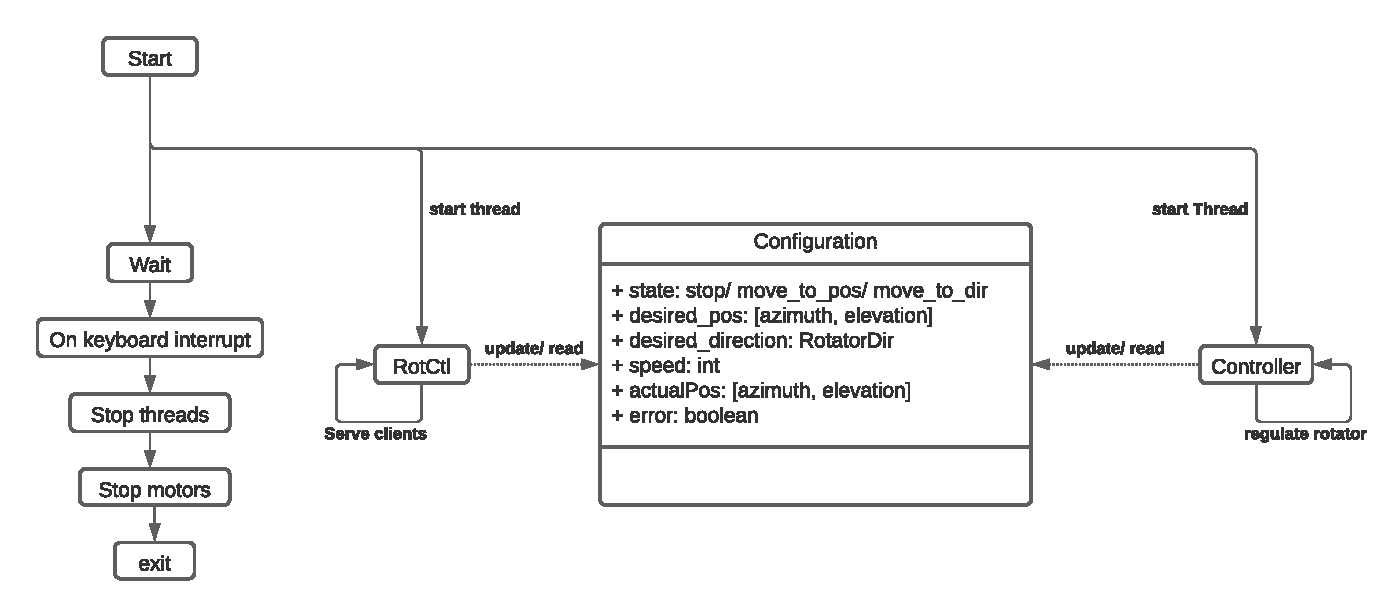
\includegraphics[width=\linewidth]{../art/Code flow chart.pdf}
	\caption{Raspberry Pi HAT flow diagram}
\end{figure}

\subsubsection{Possible improvements}
The time constrains didn't allow to make any real use of the EEPROM on the pi hat. With more time, it would be possible to save a configuration on that EEPROM, to set up pi the pi automatically. The I2C bus, for example, could be enabled, as soon as the board is plugged in.

In a demonstration video, we showed the movement of the rotator. The readings of all sensors work well. Unfortunately, more testing is required on the position calculation. As of now, we still assume some bugs in the algorithm to get the current position. The safety switches are included in the code, but not yet on the actual rotator. It's effortless to stop the rotator at any given time per command over rotctl or over the ssh connection. Playing around with it doesn't introduce a huge risk. But we don't recommend putting it up somewhere and to expect, that it doesn't break itself eventually.